
\section{Conclusions}
\label{sec:concl}

In order for the MSC to be an effective resource, it is necessary that students are able to find an available tutor when they visit. During its busiest times, though, this is not always the case. By collecting data on MSC activity with a Raspberry Pi, this project discovered that the center is busiest during evenings. Based on this information, it can be determined that students seeking help will most likely be successful if they visit the MSC between 4:00 and 6:00 (the first shift for many of the tutors) and not on Tuesday, Wednesday, or Thursday. The results also show that the amounts of light and sound in the MSC are not necessarily determinants of activity.

It is important to point out a certain degree of error in the data collection, though. Specifically, the processing of the camera data did not always accurately reflect the number of people in the room. More subtle movements would often go undetected by the computer vision algorithm, not to mention people who were sitting still (see Figure \ref{fig:cv}).

Nevertheless, this project accomplished its goal of learning more about patterns in the usage of Davidson College's Math and Science Center.

\begin{figure}[t]
    \centering
    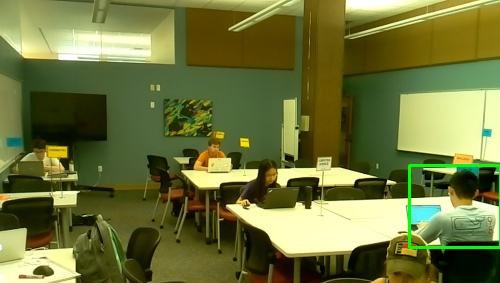
\includegraphics[width=0.97\linewidth]{figs/18-05-01-17-36-00.jpg}
    \caption{Image of MSC captured at 5:36 PM on May 1st. The green box in the bottom right of the image highlights an object that OpenCV recognized as in motion. It is evident that only one of the five people in the room was detected.}
    \label{fig:cv}
\end{figure}


